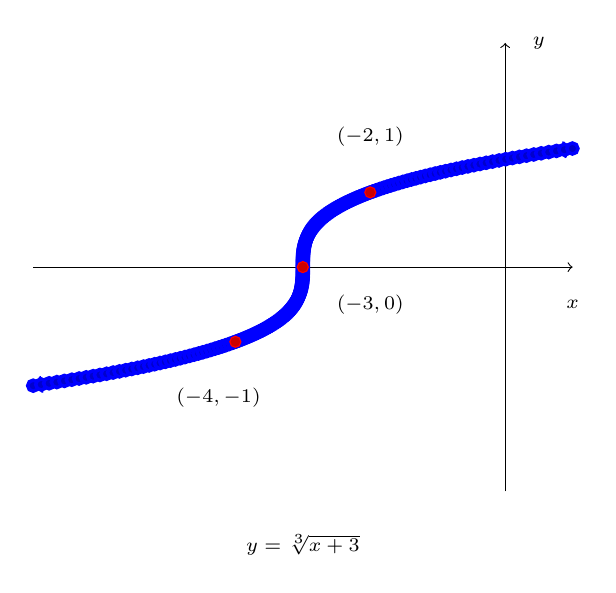
\begin{tikzpicture}
\begin{axis}[
  xmin=-7, xmax=1,
  ymin=-3, ymax=3,
  axis lines=middle,
  axis line style={->},
  ticks=none,
  clip=false
]
\node at (axis cs:1,-0.5){\scriptsize $x$};
\node at (axis cs:0.5,3){\scriptsize $y$};
\node at (axis cs:-2,1.75){\scriptsize $(-2,1)$};
\node at (axis cs:-2,-0.5){\scriptsize $(-3,0)$};
\node at (axis cs:-4.25,-1.75){\scriptsize $(-4,-1)$};

\addplot+[domain=-1.587:1.587, samples=200, smooth, line width=1.25pt, <->, variable=\t, parametric]
  ({\t^3-3},{\t});

\addplot+[only marks, mark=*, mark size=2pt] coordinates {(-2,1) (-3,0) (-4,-1)};

% Caption
\node at (rel axis cs:0.5,-0.12){\scriptsize $y=\sqrt[3]{x+3}$};
\end{axis}
\end{tikzpicture}